\documentclass{article}

\usepackage[utf8x]{inputenc}
\usepackage[english,russian]{babel}
\usepackage{graphicx}
\usepackage{amsmath}
\usepackage{amssymb}
\usepackage{extarrows}
\usepackage{vmargin}
\usepackage{MnSymbol}
\setpapersize{A4}
\setmarginsrb{2cm}{2cm}{2cm}{2cm}{0pt}{0mm}{0pt}{13mm}
%\usepackage{cmap}

\newtheorem{theorem}{Теорема}


\begin{document}

\centerline{\large Курс лекция для магистров ВМК МГУ}
\centerline {\textbf{\LARGE Обратные задачи математической физики}}
\centerline {Затехал Строков Вениамин 2025}

\vspace{0.4cm}

\centerline{\LARGE Лекция 3. Задача определение формы}

\vspace{1cm}
\centerline{\large Единственность}

Рассмотрим класс тел, имеющих средние плоскости, т.е. для них $\exists$ плоскость $P$ такая, что если $Oz \bot P$, то поверхность тела описывается уравнениями
\[
z = \varphi(x,y), z = \psi(x,y).
\]

\begin{theorem}
(единственности): \\
При постоянной известной плотности двух тел допустим, что тела обладают параллельными средними плоскостями и центры тяжести расположены внутри тел. Тогда при равенстве внешних потенциалов тела совпадают.
\end{theorem}
Доказательство:

Если
\[
v(M) = \iiint_T \dfrac{\sigma(M')}{z_{MM'}} d \tau_{M'} = 0,
\]
вне тела $T$, то $\sigma \bot \forall$ гармонической функции $u(M)$ в $T$. Действительно, из II формулы Грина имеем:
\[
\iiint_T (\Delta v u - \Delta u v) d \tau = \{\Delta u = 0\} = \iint_{\partial T} [\dfrac{\partial v}{\partial n} u - \dfrac{\partial u}{\partial n} v] ds = 0 = - 4 \pi \iiint \sigma u d\tau.
\]

Рассмотрим тело $T_1 \bigcup T_2$, для $T_1$, $T_2$, имеющих параллельные средние плоскости $z = z_1$ и $z = z_2$.
Тогда $\forall$ гармонической функции $u(M)$ в $T$:
\[
\iiint_{T = T_1 \bigcup T_2} \sigma (M) u(M) d\tau_M = 0 
\]
где
\[
\sigma(M) = 
	\begin{cases}
	1, & M \in T_1 \setminus (T_1 \bigcap T_2);\\
	0, & M \in T_1 \bigcap T_2;\\
	-1, &M \in T_2 \setminus (T_1 \bigcap T_2).
	\end{cases}
\]
т.е. $\sigma (M) = \sigma_1 - \sigma_2$ - разность плотностей.

\vspace{0.5cm}
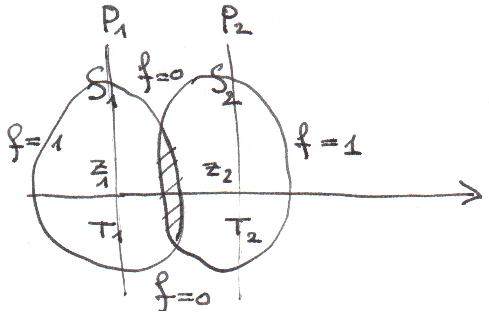
\includegraphics[scale=0.85]{pic1.png}

Рассмотрим 
\[
f(P) = 
	\begin{cases}
	1, & z < z_1, P \in S_1;\\
	1, & z > z_2, P \in S_2;\\
	0, & \text{иначе}.
	\end{cases}
\]
и поставим задачу Дирихле в $T$:
\[
\begin{cases}
\Delta F = 0, & M \in T;\\
F \bigg|_S = f, & S = \partial T.
\end{cases}
\]

Очевидно, что $\dfrac{\partial F}{\partial z}$ гармоническая в $T$. По формуле Остроградского имеем:
\[
\begin{split}
\iiint_T \sigma \dfrac{\partial F}{\partial z} dx dy dz = 
\iiint_{T_1} \sigma_1 \dfrac{\partial F}{\partial z} dx dy dz &- 
\iiint_{T_2} \sigma_2 \dfrac{\partial F}{\partial z} dx dy dz=\\
= - \iint_{S_1} F \bigg|_{z<z_1} dx dy - \iint_{S_2} F \bigg|_{z>z_2} dx dy &+ \iint_{S_1} F \bigg|_{z>z_1} dx dy + \iint_{S_2} F \bigg|_{z<z_2} dx dy = \\
= -f \bigg|_{z<z_1}|s_1| - f \bigg|_{z > z_2} |s_2| &+ F^* \bigg|_{z_>z_1} |s_1| + F^{**} \bigg|_{z_>z_2} |s_2|
\end{split}
\]
где $F^*$ - среднее по поверхности $S_1$ при $z > z_1$, $F^{**}$ - по поверхности $S_2$ при $z <z_2$, $|s_1|$, $|s_2|$ - площади сечений. Но $f \bigg|_{z<z_1} = 1, f \bigg|_{z>z_2} = 1$, а $F^* F^{**} < 1$ по принципу max, т.к. $T_1 \bigcap T_2$ - общая часть - внутренняя часть тела $T$. Это является следствием того, что центр тяжести тел совпадает и лежит внутри тел.

Таким образом:
\[
\iiint_T \sigma \dfrac{\partial F}{\partial z} d \tau = (F^{***} -1)(|s_1| + |s_2|) < 0,
\]

Противоречие! $\blacksquare$
\vspace{0.5cm}


Замечание: Для выпуклого тела цент тяжести лежит внутри тела. Пусть $O$ - центр тяжести.
\[
\begin{split}
u(M) = \iiint_T \dfrac{\rho(M')}{| \overrightarrow{r}_{M'O} + \overrightarrow{r}_{OM} |} d \tau_{M'} = 
\iiint_T \rho(M') [ \dfrac{1}{r_{OM}} + \overrightarrow{r}_{M'O} \overrightarrow{\nabla} \dfrac{1}{r_{OM}} + \mathcal{O} (\dfrac{1}{r_{OM}^3})] d\tau_{M'} = \\
=\dfrac{1}{r_{OM}} \iiint_T \rho(M') d \tau_{M'} + \dfrac{\overrightarrow{r}_{OM}}{r_{OM}^3} \iiint_T \rho(M') \overrightarrow{r}_{OM} d \tau_{M'} + \mathcal{O} (\dfrac{1}{r_{OM}^3}) = 
\dfrac{m}{r_{OM}} + \dfrac{\overrightarrow{r}_{OM}}{r_{OM}^2} \overrightarrow{\mu}_0 + \mathcal{O} (\dfrac{1}{r_{OM}^3})
\end{split}
\]

Определение: Точка $O$ такая что $\overrightarrow{\mu}_0 = 0$ называется центром тяжести тела.

Из асимптотики  потенциалов, совпадающих вне тел $u(M) \to 0$, при $M \to \infty$ получаем, что центр тяжести тел - их общая точка. Действительно, пусть $u_1(M) = u_2(M)$ вне $S_R$ и пусть $O_1$ - центр тяжести $T_1$. Тогда

\[
u_1(M) = \dfrac{m_1}{r_{O_1M}} + \dfrac{\overrightarrow{r}_{O_1M}}{r_{O_1M}^3} \overrightarrow{\mu}_{O_1}^{(1)} + \mathcal{O}(\dfrac{1}{r_{O_1M}^3}), 
\overrightarrow{\mu}_{O_1}^{(1)} = 0;
\]

но тогда из совпадения разложений $ \overrightarrow{\mu}_{O_1
}^{(2)} = 0 $, т.е. $ O_1 = O_2 $.


\vspace{1cm}
\centerline{\large Обратная задача для полуплоскости}

\vspace{0.5cm}
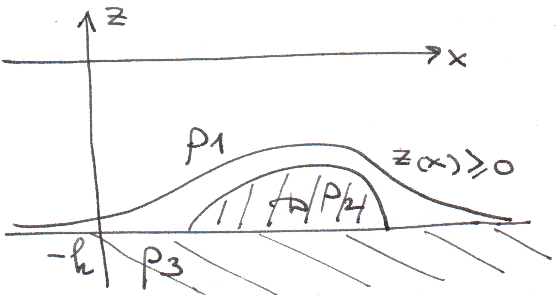
\includegraphics[scale=0.85]{pic2.png}

Если $z(x)$ не финитная, то ОЗ может иметь более одного решения.
На земной поверхности регистрируется аномалия поля тяжести $g(x)$ для потенциала $u(x,z)$:
\[
v(x) = u(x,z) \bigg|_{z = 0} = (\rho_2 - \rho_1) \iint_D \ln \dfrac{1}{\sqrt{(x-\xi)^2 + (z - \eta)^2}} \bigg|_{z=0} d\xi d\eta.
\]

Получим интегральное уравнение, считая известной $g(x)$:
\[
-g(x) = \dfrac{\partial u}{\partial z} \bigg|_{z = 0} = \rho \dfrac{\partial}{\partial z} \int_{-\infty}^{\infty} \int_{-h}^{z(\xi)-h} \dfrac{1}{2} \ln \dfrac{1}{(x-\xi)^2 + (z - \eta)^2} \bigg|_{z=0} d\xi d\eta = \{ \dfrac{\partial}{\partial z} =
 - \dfrac{\partial}{\partial \eta} \} =
\]
\[
= -\rho \int_{-\infty}^{\infty} \int_{-h}^{z(\xi)-h} \dfrac{\partial}{\partial \eta} \dfrac{1}{2} \ln \dfrac{1}{(x-\xi)^2 + (z - \eta)^2} \bigg|_{z=0} d\xi d\eta =
 \dfrac{\rho}{2} \int_{-\infty}^{\infty} \ln \dfrac{(x-\xi)^2 + (z(\xi) - h)^2}{(x-\xi)^2 + h^2} d\xi.
\]

Если $z(\xi)$ - финитна, то из асимптотики $v(x)$ при $x \rightarrow \infty$ определяется $h \rho S_D = hm$.

Рассмотрим случай $|z(\xi)| << h$. Тогда 
\[
\ln \dfrac{(x-\xi)^2 + (z(\xi) - h)^2}{(x-\xi)^2 + h^2} \approx 
\ln \dfrac{(x-\xi)^2 + h^2 - 2z(\xi)h}{(x-\xi)^2 + h^2} \approx
-\dfrac{2hz(\xi)}{(x-\xi)^2 + h^2} \Rightarrow
\]
\[
g(x) = \rho h \int_{-\infty}^{\infty} \dfrac{z(\xi)}{(x-\xi)^2 + h^2} d\xi,
\]
это интегральное уравнение с ядром Коши. Пусть $z(\xi) = 0$ вне $[0,a]$. Тогда
\[
g(x) = \rho h \int_{0}^{a} \dfrac{z(\xi)}{(x-\xi)^2 + h^2} d\xi,
\]
при $x \rightarrow \infty$ находим $\rho h S_D$.

Исследуем вопрос о единственности определения $z(x)$ при известном $\rho h$, если $g(x)$ известна при $x \in \mathbb{R}$.
\[
\int_{-\infty}^{\infty} \dfrac{z(\xi)}{(x-\xi)^2 + h^2} d\xi = 0,
\]
и, поскольку $z(\xi)$ финитна, можно совершить преобразование Фурье для интеграла свертки. Получаем
\[
\dfrac{\pi}{2h} \tilde{z}(\omega) e^{-|\omega|h} = 0 \Rightarrow \tilde{z}(\omega) = 0.
\]
Таким образом, $z(x)$, $x \in [0,a]$определяется однозначно.

Если $g(x)$ известна на $[c,d]$, то в силу аналитичности она известна и на $\mathbb{R} \Rightarrow$  единственность решения ОЗ.

Решим ОЗ с помощью метода регуляризации. Пусть $Z \equiv \overset{\circ}{W_2^1}[0,a]$, $U = L_2[c,d]$; $\overset{\circ}{W_2^1} = \overset{\circ}{H^1}$
\[
A z = \int_{0}^{a} \dfrac{z(\xi)}{(x-\xi)^2 + h^2} d\xi = u(x), \hspace{0.5cm} x \in [c,d], [0,a] \subset [c,d]
\]

Из минимуиа функционала Тихонова $M^{\alpha} [x,u] = \lVert Az - u \rVert_{L_2[c,d]}^2 + \alpha \lVert z \rVert_{\overset{\circ}{W_2^1}[0,a]}^2$ имеем  $(A^* A + \alpha E)z = A^* u$, где $A^*$ - сопряжённый оператор, $A^* : L_2[c,d] \rightarrow \overset{\circ}{W_2^1}[0,a]$ определяется из $(A \varphi, \psi)_{L_2[c,d]} = \{A^* \psi = y\} = (\varphi, A^* \psi)_{\overset{\circ}{W_2^1}[0,a]}, \forall \varphi \in \overset{\circ}{W_2^1}[0,a], \psi \in L_2$.
\[
\int_c^d \int_0^a K(x,s) \varphi(s) ds \psi(x) dx = 
\int_0^a [ \varphi(s) y(s) + \varphi'(s) y'(s)] ds =
\int_0^a \varphi(s) \int_c^d K(x,s) \psi(x) dx ds =
\]
\[
= \varphi(s) y'(s) \bigg|_0^a + \int_0^a \varphi(s)(y(s) - y''(s))ds, \hspace{1cm}
\forall \varphi \in \overset{\circ}{W_2^1}[0,a], \forall \psi \in L_2[c,d] \Rightarrow
\]

\[
\begin{cases}
y''(s) - y(s) = - \int_c^d K(x,s) \psi(x)dx = f(x)  \Leftrightarrow A^* \psi = y \in \overset{\circ}{W_2^1}[0,a]; \\
y(0) = y(a) = 0.
\end{cases}
\]
$G(s,t)$ - функция Грина первой краевой задачи $y(s) = \int_0^a G(s,t) f(t) dt$. Из уравнения Эйлера имеем:
\[
\alpha z(s) + \int_0^a G(s,t) \int_c^d K(x,t) \int_0^a K(x,\xi) z(\xi) d\xi dx dt = 
- \int_0^a G(s,t) \int_c^d K(x,t) u(x) dx dt
\]
или
\[
\alpha z(s) + \int_0^a \int_0^a G(s,t) B(t,\xi) z(\xi) d\xi dt = -\int_0^a G(s,t) f(t)dt.
\]
\[
B(t,\xi) = \int_c^d K(x,t) K(x, \xi) dx, \hspace{0.5cm} f(t) = \int_c^d K(x,t) u(x) dx/
\]
$\alpha$ выбирается в соответствии с теоремами $\alpha(\delta) - \lVert A z_{\alpha(\delta)} - u \delta \rVert = \delta$ - принцип невязки. Сходимость в  $\overset{\circ}{W_2^1}[0,a] \Rightarrow$ в $C[0,a]$.



\end{document}